\documentclass{standalone}
\usepackage{tikz}
\usepackage{ctex,siunitx}
\setCJKmainfont{Noto Serif CJK SC}
\usepackage{tkz-euclide}
\usepackage{amsmath}
\usetikzlibrary{patterns, calc}
\usetikzlibrary {decorations.pathmorphing, decorations.pathreplacing, decorations.shapes,}

\begin{document}
\small
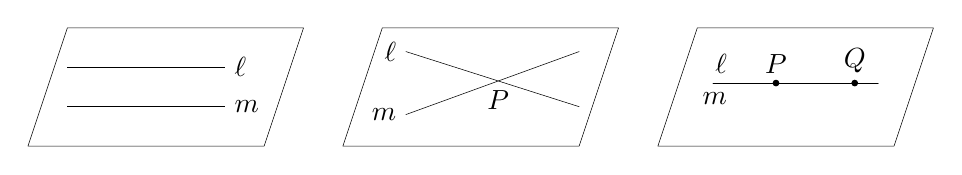
\begin{tikzpicture}[>=stealth,scale=1]
  \tkzSetUpPoint[fill=black]
  % \useasboundingbox(-1,-0.75)rectangle(3.7,1.4);
  \begin{scope}
    \tkzDefPoints{0/0/A, 3/0/B, 3.5/1.5/C}
    \tkzDefPointsBy[translation = from B to C](A){D}
    \tkzDrawPolygon(A,B,C,D)
    \draw(.5,.5)--(2.5,.5)node[right]{$m$};
    \draw(.5,1)--(2.5,1)node[right]{$\ell$};
  \end{scope}
  \begin{scope}[xshift=4cm]
    \tkzDefPoints{0/0/A, 3/0/B, 3.5/1.5/C}
    \tkzDefPointsBy[translation = from B to C](A){D}
    \tkzDrawPolygon(A,B,C,D)
    \tkzDefPoints{.8/1.2/A, 3/.5/B, .8/.4/C, 3/1.2/D}
    \tkzInterLL(A,B)(C,D)\tkzGetPoint{P}
    \tkzLabelPoints[below](P)
    \tkzLabelPoint[left](A){$\ell$}
    \tkzLabelPoint[left](C){$m$}
    \tkzDrawSegments(A,B C,D)
  \end{scope}
  \begin{scope}[xshift=8cm]
    \tkzDefPoints{0/0/A, 3/0/B, 3.5/1.5/C}
    \tkzDefPointsBy[translation = from B to C](A){D}
    \tkzDrawPolygon(A,B,C,D)
    \tkzDefPoints{1/.8/P', 1.5/.8/P, 2.5/.8/Q}
    \tkzDrawLine(P',Q)
    \tkzDrawPoints(P,Q)
    \tkzLabelPoints[above](P,Q)
    \tkzLabelPoint[above left](P'){$\ell$}
    \tkzLabelPoint[below left](P'){$m$}
  \end{scope}
\end{tikzpicture}
\end{document}